\documentclass[12pt]{extarticle} 
\usepackage{unicode-math}
\usepackage{amsthm,graphicx,xcolor,natbib,enumitem,booktabs,tabularx}
%\usepackage[paperwidth=126mm, paperheight=96mm, top=5mm, bottom=5mm, right=5mm, left=5mm]{geometry}
\usepackage[margin=1cm,footskip=5mm]{geometry}
\pagenumbering{gobble}

\usepackage[BoldFont,SlantFont]{xeCJK}  
\xeCJKsetemboldenfactor{2}
\setCJKmainfont{cwTeX Q Yuan Medium}
%\setCJKmainfont{cwTeX Q Kai Medium}
%\setCJKmainfont{cwTeX Q Ming Medium}
%\setCJKmainfont[AutoFakeSlant=.1,AutoFakeBold=1]{cwTeX Q Kai Medium} 
%\setCJKfamilyfont{kaiv}[Vertical=RotatedGlyphs]{cwTeX Q Medium}
%\setmainfont{texgyrepagella-regular.otf}
%\setmathfont{texgyrepagella-math.otf}
\newcommand{\ds}{\displaystyle}
\newcommand{\ie}{\;\Longrightarrow\;}
\newcommand{\ifff}{\;\Longleftrightarrow\;}
\newcommand{\orr}{\;\vee\;}
\newcommand{\andd}{\;\wedge\;}
\newcommand{\mi}{\mathrm{i}}
\DeclareMathOperator*{\dom}{dom}
\DeclareMathOperator*{\codom}{codom}
\DeclareMathOperator*{\ran}{ran}
\newcommand{\floor}[1]{\lfloor #1 \rfloor}
\newcommand{\ceil}[1]{\lceil #1 \rceil}

\newcommand{\bdiff}[2]{ \frac{\mathrm{d}}{\mathrm{d}#2} \left( #1 \right)}
\newcommand{\ddiff}[3]{ \frac{\mathrm{d}^#1#2}{\mathrm{d}{#3}^#1}}
\newcommand{\half}{\tfrac{1}{2}}
\newcommand{\diff}[2]{ \frac{\mathrm{d}\hfil#1\hfil}{\mathrm{d}#2}}
\newcommand{\difftwo}[2]{ \frac{\mathrm{d^2}\hfil#1\hfil}{\mathrm{d}{#2}^2}}

% figure --> 圖
\renewcommand{\appendixname}{附錄}
\renewcommand{\figurename}{圖}
\renewcommand{\tablename}{表}
\renewcommand{\refname}{參考文獻}

\usepackage{hyperref}
\hypersetup{
    colorlinks,
    linkcolor={red!50!black},
    citecolor={blue!60!black},
    urlcolor={blue!60!black}
    %urlcolor={blue!80!black}
}

\theoremstyle{definition}
\newtheorem*{dfn}{定義}
\newtheorem*{prp}{性質}
\newtheorem*{fact}{結論}
\newtheorem*{thm}{定理}
\newtheorem*{ex}{例}
\newtheorem*{sol}{解}
\newtheorem*{prf}{證}
\newtheorem*{rmk}{註}
\newtheorem*{exe}{習題}

%\setenumerate{label=(\roman*),itemsep=1pt,topsep=3pt}
\newcommand{\myline}{\noindent\makebox[\linewidth]{\rule{\paperwidth}{0.4pt}}}
%\newcommand{\myline}{\textcolor[RGB]{220,220,220}{\rule{\linewidth}{1pt}}}

%%%%%%%%%%%%%%%%%%%%%%%%%%%%%%%%%%%%%%%%%%%%%%%%%%%%%%%%%%%%%%%%%%%%%
% colorblind-friendly palette
% mixed colours: CB sees contrasting grays
\definecolor{M1}{RGB}{0,0,0}
\definecolor{M2}{RGB}{0,73,73}
\definecolor{M3}{RGB}{0,146,146}
\definecolor{M4}{RGB}{255,109,182}
\definecolor{M5}{RGB}{255,182,119}
% cool colours: CB sees contrasting blues
\definecolor{C1}{RGB}{73,0,146}
\definecolor{C2}{RGB}{0,109,219}
\definecolor{C3}{RGB}{182,109,255}
\definecolor{C4}{RGB}{109,182,255}
\definecolor{C5}{RGB}{182,219,255}
% warm colours: CB sees contrasting yellow
\definecolor{W1}{RGB}{146,0,0}
\definecolor{W2}{RGB}{146,73,0}
\definecolor{W3}{RGB}{219,209,0}
\definecolor{W4}{RGB}{36,255,36}
\definecolor{W5}{RGB}{255,255,109}

%%%%%%%%%%%%%%%%%%%%%%%%%%%%%%%%%%%%%%%%%%%%%%%%%%%%%%%%%%%%%%%%%%%%%

\usepackage{multicol}
\usepackage{tikz}
\usetikzlibrary{arrows.meta,angles,quotes}
\usepackage{pgfplots}
% axis style, ticks, etc
\pgfplotsset{every axis/.append style={
                   label style={font=\fontsize{4}{4}\selectfont},
                   tick label style={font=\fontsize{4}{4}\selectfont}  
               },
            }
\renewcommand\tabularxcolumn[1]{m{#1}}

\usepackage{fancyhdr}
\fancypagestyle{firststyle} {
   \fancyhf{}
   \fancyfoot[R]{\footnotesize \DTMnow}
   \renewcommand{\headrulewidth}{0pt} 
}
\usepackage{datetime2}
\usepackage{calc}
\def\theyear{\the\year}

\usepackage{etoolbox}
\newbool{invsec}
\booltrue{invsec}


% \sector solution
% https://tex.stackexchange.com/questions/310384/is-there-a-latex-symbol-that-looks-like-a-sector-of-a-circle
\usepackage{pgf}

\newcommand*{\SectorRadius}{3mm}
\newcommand*{\SectorHalfAngle}{30}
\newcommand*{\SectorLineWidth}{.7pt}

\newcommand*{\sector}{%
  \begin{pgfpicture}
    \pgfpathmoveto{\pgforigin}%
    \pgfpathlineto{\pgfpointpolar{90-(\SectorHalfAngle)}{\SectorRadius}}%
    \pgfarc{90-(\SectorHalfAngle)}{90+\SectorHalfAngle}{\SectorRadius}%
    \pgfpathclose
    \pgfsetlinewidth{\SectorLineWidth}%
    \pgfusepath{stroke}%
  \end{pgfpicture}%
}

\begin{document}
\title{\texorpdfstring{\vspace{-16mm} 第二章\ \ 微分}{第二章\ \ 微分}} 
\author{\vspace{-5em}}
\date{\vspace{-5em}}
\maketitle
\thispagestyle{firststyle}

%\newpage

\section*{2.1 導數與導函數}

\begin{minipage}{0.3\textwidth}
  %\begin{figure}[!htbp]
  %  \centering
  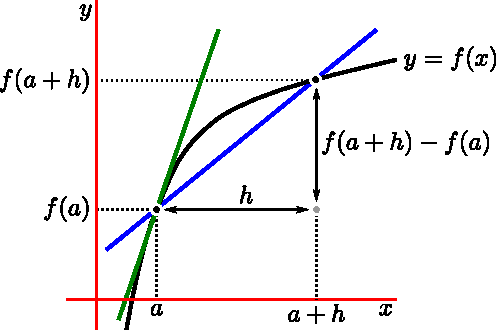
\includegraphics[scale=0.75,page=1]{fig/tangentA.pdf}
  %\end{figure}
\end{minipage}
\quad
\begin{minipage}{0.65\textwidth}
  \begin{dfn}
    給定 $f(x)$, $a\in\dom f$. $f$ 在 $a$ 的導數 (derivative) $f'(a)$ 定義為 $$f'(a) = \lim_{h\to 0}\frac{f(a + h) - f(a)}{h}$$ 若 $f'(a)$ 存在, 則稱 $f$ 在 $a$ 可微(分)(differentiable). $f$ 的導函數 $f'(x)$ 定義為 $$f'(x) = \lim_{h\to 0}\frac{f(x + h) - f(x)}{h}$$ 
    %\end{itemize}
  \end{dfn}
\end{minipage}

\begin{rmk}
  \begin{itemize}\setlength\itemsep{0em}
    \item[]
    \item 求導函數之過程稱為微分 (differentiation) : 求 $f'(x)$ $\ifff$ $f(x)$ (對 $x$) 微分
    \item 給定 $y = f(x)$, 其導函數可記為 $\ds f'(x) = f' = y' = \frac{\text{d}y}{\text{d}x} = \frac{\text{d}f}{\text{d}x} = \frac{\text{d}}{\text{d}x} f(x) = Df(x) = D_x f(x)$. 
    \item $f$ 在 $a$ 的導數可記為 $\ds f'(a) = \frac{\text{d}y}{\text{d}x}\,\bigg|_{\,x = a}$.  
  \end{itemize}
\end{rmk}

\begin{ex}
  以極限定義求以下 $f(x)$ 之導函數 $f'(x)$, 當 $f(x)$ 為 
  \setlength{\columnsep}{-3mm}
  \begin{multicols}{8}
    \begin{enumerate}\setlength\itemsep{0em}
      %\item $x$ 
      \item $x^2$
      \item $x^4$
      \item $\frac{1}{x}$ 
      \item $\frac{1}{x^5}$
      \item $\frac{1}{x^2 + 3}$
      \item $\sqrt{x + 1}$
      \item $\sqrt{x^2 + 1}$
      \item $\sqrt[3]{1 - x^3}$
    \end{enumerate}
  \end{multicols}
\end{ex}

\begin{sol}
  \begin{enumerate}\setlength\itemsep{0em}
    \item[]
    %\item $\ds f'(x) = \lim_{h\to 0}\frac{(x + h) - x}{h} = \lim_{h\to 0}\frac{h}{h} = \lim_{h\to 0}\,1 = 1$. 
    \item $\ds f'(x) = \lim_{h\to 0}\frac{(x + h)^2 - x^2}{h} = \lim_{h\to 0}\frac{2 x h + h^2}{h} = \lim_{h\to 0}\,(2x + h) = 2x$. 
    \item $\ds f'(x) = \lim_{h\to 0}\frac{(x + h)^4 - x^4}{h} = \lim_{h\to 0}\frac{4 x^3 h + 6x^2 h^2 + 4 x h^3 + h^4}{h} = \lim_{h\to 0}\,(4x^3 + 6x^2 h + 4 x h^2 + h^3) = 4x^3$. 
    \item $\ds f'(x) = \lim_{h\to 0}\frac{\frac{1}{x + h} - \frac{1}{x}}{h} = \lim_{h\to 0}\frac{x - (x + h)}{h\,(x + h)\,x} = \lim_{h\to 0}\frac{-h}{h\,(x + h)\,x} = \lim_{h\to 0}\frac{-1}{(x + h)\,x} = \frac{-1}{x^2} = (-1)\,x^{-2}$. 
    \item $\ds f'(x) = \lim_{h\to 0}\frac{\frac{1}{(x + h)^5} - \frac{1}{x^5}}{h} = \lim_{h\to 0}\frac{x^5 - (x + h)^5}{h\,(x + h)^5\,x^5} \\ = \lim_{h\to 0}\frac{(-h)(x^4 + x^3(x + h) + x^2(x + h)^2 + x^3(x + h) + (x + h)^4)}{h\,(x + h)^5\,x^5}\\ = \lim_{h\to 0}\frac{-(x^4 + x^3(x + h) + x^2(x + h)^2 + x^3(x + h) + (x + h)^4)}{(x + h)^5\,x^5} = \frac{-5x^4}{x^{10}} = \frac{-5}{x^6} = (-5)\,x^{-6}$. 
   \item $\ds f'(x) = \lim_{h\to 0}\frac{\frac{1}{(x + h)^2 + 3} - \frac{1}{x^2 + 3}}{h} = \lim_{h\to 0}\frac{(x^2 + 3) - ((x + h)^2 + 3)}{h\,((x + h)^2 + 3)\,(x^2 + 3)} = \lim_{h\to 0}\frac{(2x + h)\,(-h)}{h\,((x + h)^2 + 3)\,(x^2 + 3)} \\ = \lim_{h\to 0}\frac{-(2x + h)}{((x + h)^2 + 3)(x^2 + 3)} = \frac{-2x}{(x^2 + 3)^2}$. 
   \item $\ds f'(x) = \lim_{h\to 0}\frac{\sqrt{x + h + 1} - \sqrt{x + 1}}{h} = \lim_{h\to 0}\frac{h}{h\,(\sqrt{x + h + 1} + \sqrt{x + 1})} = \frac{1}{2\sqrt{x + 1}}$. 
   \item $\ds f'(x) = \lim_{h\to 0}\frac{\sqrt{(x + h)^2 + 1} - \sqrt{x^2 + 1}}{h} = \lim_{h\to 0}\frac{h\,(2x + h)}{h\,(\sqrt{(x + h)^2 + 1} + \sqrt{x^2 + 1})} = \frac{x}{\sqrt{x^2 + 1}}$. 
   \item $\ds f'(x) = \lim_{h\to 0}\frac{\sqrt[3]{1 - (x + h)^3} - \sqrt[3]{1 - x^3}}{h}\qquad\qquad(\text{使用}\;a^3 - b^3 = (a - b)(a^2 + ab + b^2)) \\= \lim_{h\to 0}{\frac{1 - (x + h)^3 - (1 - x^3)}{h\,\big(\big(\sqrt[3]{1 - (x + h)^3}\big)^2 + \sqrt[3]{1 - (x + h)^3}\,\sqrt[3]{1 - x^3} + \big(\sqrt[3]{1 - x^3}\big)^2\big)}} \\
     = \lim_{h\to 0}\frac{(-h)(x^2 + x(x + h) + (x + h)^2)}{h\,\big(\big(\sqrt[3]{1 - (x + h)^3}\big)^2 + \sqrt[3]{1 - (x + h)^3}\,\sqrt[3]{1 - x^3} + \big(\sqrt[3]{1 - x^3}\big)^2\big)} = \frac{-3x^2}{3\big(\sqrt[3]{1 - x^3}\big)^2} = \frac{-x^2}{\big(\sqrt[3]{1 - x^3}\big)^2}$. 
  \end{enumerate}
\end{sol}

\begin{fact}
  $x^\alpha$ ($\alpha\in\mathbb{R}$) 之導函數為 $\alpha\,x^{\alpha - 1}$. 
\end{fact}

\begin{dfn}
  %\begin{itemize}\setlength\itemsep{0em}
    %\item[]
    %\item 
      若 $f$ 在 $(a, b)$ 上每一點均有導數, 則稱 $f$ 在 $(a, b)$ 可微 (分) . 
    %\item $f$ 在 $a$ 的右導數 $f'_+(a)$ 定義為 $\ds f'_+(a) = \lim_{h\to 0+}\frac{f(a + h) - f(a)}{h}$; \\$f$ 在 $a$ 的左導數 $f'_-(a)$ 定義為 $\ds f'_-(a) = \lim_{h\to 0-}\frac{f(a + h) - f(a)}{h}$. 
    %\item 若 $f$ 在 $(a, b)$ 可微, 在 $a$ 有右導數, 在 $b$ 有左導數, 則稱 $f$ 在 $[a, b]$ 可微 (分) . 
  %\end{itemize}
\end{dfn}

\begin{thm}
  若 $f$ 在 $a$ 可微, 則 $f$ 在 $a$ 連續. 
\end{thm}

%\begin{rmk}
%  \begin{itemize}\setlength\itemsep{0em}
%    \item[]
%    \item $f$ 在 $a$ 不可微之三情形: 
%      \begin{itemize}\setlength\itemsep{0em}
%        \item $f$ 在 $a$ 不連續. 
%        \item $f$ 在 $a$ 連續, $\ds f'_+(a)\ne f'_-(a)$: $a$ 為拐點 (corner, kink) . 
%        \item $f$ 在 $a$ 連續, $\ds\lim_{x\to a}|f'(x)| = \infty$: $a$ 為臍點 (cusp) , 有垂直切線. 
%      \end{itemize}
%    \item 
%      \begin{itemize}\setlength\itemsep{0em}
%        \item 連續函數不一定可微.  ($f(x) = |x|$ 在 $x = 0$ 處) 
%        \item 若 $f$ 在 $a$ 可微, 則在 $a$ 必有切線. 
%        \item $f$ 在 $a$ 有切線, $f$ 在 $a$ 未必可微 (垂直切線) . 
%      \end{itemize}
%  \end{itemize}
%\end{rmk}

\section*{2.2 微分規則}

\begin{thm}[四則運算] 令 $f$, $g$ 可微, $c\in\mathbb{R}$. 則
  \setlength{\columnsep}{-0mm}
  \begin{multicols}{3}
    \begin{enumerate}\setlength\itemsep{0em}
      \item $\ds (c)' = 0$
      \item $\ds (c\,f)' = c\,f'$
      \item $\ds (f\pm g)' = f'\!\pm g'$
      \item $\ds (f\cdot g)' = f'\!\cdot g + f\cdot g'$
      \item $\ds \Big(\frac{f}{g}\Big)' = \frac{g\cdot f' - g'\!\cdot f}{g^2}$
    \end{enumerate}
  \end{multicols}
\end{thm}

\begin{ex} 求導函數. 
  \begin{multicols}{4}
    \begin{enumerate}\setlength\itemsep{0em}
      \item $x^5$
      \item $\frac{1}{x^2 + 3}$
      \item $\frac{x - 1}{x + 1}$
      \item $\sqrt{\frac{x - 1}{x + 1}}$
    \end{enumerate}
  \end{multicols}
\end{ex}

\begin{sol}
  \begin{enumerate}\setlength\itemsep{0em}
    \item[]
    \item $\ds (x^5)' = (x \cdot x^2 \cdot x^2)' = (x)'\cdot x^2 \cdot x^2 + x\cdot(x^2)'\cdot x^2 + x\cdot x^2\cdot(x^2)' = x^4 + x\cdot(2x)\cdot x^2 + x^3\cdot(2x) = 5 x^4$
    \item $\ds\Big(\frac{1}{x^2 + 3}\Big)' = \frac{(x^2 + 3)\cdot(1)' - (x^2 + 3)'\cdot 1}{(x^2 + 3)^2} = \frac{-2x}{(x^2 + 3)^2}$
    \item $\ds\Big(\frac{x - 1}{x + 1}\Big)' = \frac{(x + 1)\cdot(x - 1)' - (x + 1)'\cdot(x - 1)}{(x + 1)^2} = \frac{2}{(x + 1)^2}$ 
    \item $\ds\bigg(\sqrt{\frac{x - 1}{x + 1}}\bigg)' = \bigg(\frac{\sqrt{x - 1}}{\sqrt{x + 1}}\bigg)' = \frac{\sqrt{x + 1}\cdot(\sqrt{x - 1})' - (\sqrt{x + 1})'\cdot\sqrt{x - 1}}{(\sqrt{x + 1})^2} \\= \frac{\sqrt{x + 1}\cdot\frac{1}{2\sqrt{x - 1}} - \frac{1}{2\sqrt{x + 1}}\cdot\sqrt{x - 1}}{(\sqrt{x + 1})^2} = \frac{\sqrt{x + 1}\cdot\sqrt{x + 1} - \sqrt{x - 1}\cdot\sqrt{x - 1}}{2\sqrt{x - 1}(\sqrt{x + 1})^3} = \frac{1}{\sqrt{(x - 1)(x + 1)^3}}$ %= \frac{1}{\sqrt{x - 1}(\sqrt{x + 1})^3} 
  \end{enumerate}
\end{sol}

\begin{thm}[鏈鎖律 (chain rule) ]
  若 $f(u)$ 在 $u = g(x)$ 可微, $g(x)$ 在 $x$ 可微, 則 $f\circ g$ 在 $x$ 可微: 
  \begin{align*}
    (f\circ g)'(x)\,\equiv\,(f(g(x)))' = f'(g(x))\cdot g'(x)
  \end{align*}
\end{thm}

\begin{ex} 求導函數.
  \begin{multicols}{4}
    \begin{enumerate}\setlength\itemsep{0em}
      \item $(x^3 - 1)^{\theyear}$
      \item $\sqrt{x^2 + 1}$
      \item $\frac{1}{x^2 + 3}$
      \item $\sqrt{\frac{x - 1}{x + 1}}$
    \end{enumerate}
  \end{multicols}
\end{ex}

\begin{sol}
  \begin{enumerate}\setlength\itemsep{0em}
    \item[]
    \item 令 $\ds f(u) = u^{\theyear}$, $g(x) = x^3 - 1$, 則 $\ds f'(u) = \theyear\,u^{\the\numexpr\theyear-1\relax}$, $\ds(x^3 - 1)^{\theyear} = f(g(x))$. \\由鏈鎖律 $\ds((x^3 - 1)^{\theyear})' = (f(g(x)))' = f'(g(x))\cdot g'(x) = \theyear\cdot(x^3 - 1)^{\the\numexpr\theyear-1\relax}\cdot(3x^2)$. 
    \item 令 $\ds f(u) = \sqrt{u} = u^{\frac{1}{2}}$, $g(x) = x^2 + 1$, 則 $\ds f'(u) = \frac{1}{2\sqrt{u}}$, $\ds\sqrt{x^2 + 1} = f(g(x))$. \\由鏈鎖律 $\ds (\sqrt{x^2 + 1})' = (f(g(x)))' = f'(g(x))\cdot g'(x) = \frac{1}{2\sqrt{x^2 + 1}}\cdot(2x) = \frac{x}{\sqrt{x^2 + 1}}$. 
    \item 令 $\ds f(u) = \frac{1}{u}$, $g(x) = x^2 + 3$, 則 $\ds f'(u) = \frac{-1}{u^2}$, $\ds\frac{1}{x^2 + 3} = f(g(x))$. \\由鏈鎖律 $\ds\Big(\frac{1}{x^2 + 3}\Big)' = (f(g(x)))' = f'(g(x))\cdot g'(x) = \frac{-1}{(x^2 + 3)^2}\cdot(x^2 + 3)' = \frac{-2x}{(x^2 + 3)^2}$. 
    \item 令 $\ds f(u) = \sqrt{u}$, $\ds g(x) = \frac{x - 1}{x + 1}$, 則 $\ds f'(u) = \frac{1}{2\sqrt{u}}$, $\ds\sqrt{\frac{x - 1}{x + 1}} = f(g(x))$. \\由鏈鎖律 $\ds\bigg(\sqrt{\frac{x - 1}{x + 1}}\bigg)' = (f(g(x)))' = f'(g(x))\cdot g'(x) = \frac{1}{2\sqrt{\frac{x - 1}{x + 1}}}\cdot\Big(\frac{x - 1}{x + 1}\Big)' = \frac{1}{2\sqrt{\frac{x - 1}{x + 1}}}\frac{2}{(x + 1)^2} = \frac{1}{\sqrt{(x - 1)(x + 1)^3}}$. 
  \end{enumerate}
\end{sol}

\begin{fact}
  若 $f(g(x)) = x$, 等式兩邊對 $x$ 微分 $\ie$ $\ds(f(g(x)))' = 1$ $\ie$ $\ds f'(g(x))\cdot g'(x) = 1$ $\ie$ $\ds g'(x) = \frac{1}{f'(g(x))}$.   
\end{fact}

\begin{ex}
  $f$, $g$ 為可微函數且 $\ds f(g(x)) = x$. 若 $\ds f'(x) = 1 + (f(x))^2$, 求 $g'(x)$.   
\end{ex}

\begin{sol}
  $\ds f(g(x)) = x$ 等式兩邊對 $x$ 微分得 $\ds f'(g(x))\cdot g'(x) = 1$ $\ie$ $\ds g'(x) = \frac{1}{f'(g(x))}$ $=$ $\ds\frac{1}{1 + (f(g(x)))^2}$ $=$ $\ds\frac{1}{1 + x^2}$. 
\end{sol}

\begin{ex}
  令 $\ds f(x) = e^x + x$, 求 $\ds (f^{-1})'(e + 1)$. 
\end{ex}

\begin{sol}
  令 $\ds g(x) = f^{-1}(x)$, 則 $\ds g(f(x)) = f^{-1}(f(x)) = x$. 等式兩邊對 $x$ 微分得 $\ds g'(f(x))\cdot f'(x) = 1$ $\ie$ $\ds g'(f(x)) = \frac{1}{f'(x)}$. 由 $f(1) = e + 1$, $\ds g'(e + 1) = g'(f(1)) = \frac{1}{f'(1)} = \frac{1}{e + 1}$. 
\end{sol}

%\begin{ex}
%  若 $F(x) = f(x\cdot f(x\cdot f(x)))$, 且 $f(1) = 2$, $f(2) = 3$, $f'(1) = 4$, $f'(2) = 5$, $f'(3) = 6$, 求 $F'(1)$. 
%\end{ex}
%
%\begin{sol}
%  由鏈鎖律 $\ds\big(f(x\cdot f(x\cdot f(x)))\big)' = f'(x\cdot f(x\cdot f(x)))\cdot(x\cdot f(x\cdot f(x)))'$. 又 $\ds(x\cdot f(x\cdot f(x)))' = f(x\cdot f(x)) + x\cdot f'(x\cdot f(x))\cdot(x\cdot f(x))' =  f(x\cdot f(x)) + x\cdot f'(x\cdot f(x))\cdot(x\cdot f'(x) + f(x))$. 故 $\ds F'(1) = \big(f(x\cdot f(x\cdot f(x)))\big)'\,\big|_{x = 1} = f'(x\cdot f(x\cdot f(x)))\cdot\big(f(x\cdot f(x)) + x\cdot f'(x\cdot f(x))\cdot(x\cdot f'(x) + f(x))\big)\,\big|_{x = 1} = f'(f(f(1)))\cdot\big(f(f(1)) + f'(f(1))\cdot(f'(1) + f(1))\big) = 6\cdot\big(3 + 5\cdot(4 + 2)\big) = 198$. 
%\end{sol}

\section*{2.3 自然指數, 對數與微分}

\begin{dfn}[自然指數 $e$ 與 $e^x$ 微分]
  \begin{itemize}\setlength\itemsep{0em}
    \item[]
    \item 給定 $a > 0$, 求 $f(x) = a^x$ 之導函數
    \item $\ds\diff{f}{x}=\lim_{h \to 0} \frac{f(x+h) - f(x)}{h} = \lim_{h \to 0} \frac{a^{x+h} - a^x}{h} = \lim_{h \to 0} a^x \cdot \frac{a^{h} - 1}{h} = a^x \cdot \lim_{h \to 0} \frac{a^{h} - 1}{h} = a^x\cdot C(a)$
    \item 觀察: $C(a)$ 隨 $a$ 遞增; 存在 $\frac{27}{10} < e < \frac{68}{25}$ 使 $C(e) = 1$. 
      \begin{table}[!htbp]
        \centering
        \scalebox{0.96}{
        \begin{tabular}{cccccccc}
        \toprule
        $h$ & $10^{-1}$ & $10^{-2}$ & $10^{-3}$ & $10^{-4}$ & $10^{-5}$ & $10^{-6}$ & $10^{-7}$ \\
        \midrule
        \addlinespace[1mm]
        $\ds\frac{2^h-1}{h}$ & 0.7177 & 0.6956 & 0.6934 & 0.6932 & 0.6931 & 0.6931 & 0.6931 \\
        \addlinespace[1mm]
        $\ds\frac{(\frac{5}{2})^h-1}{h}$ & 0.9596 & 0.9205 & 0.9167 & 0.9163 & 0.9163 & 0.9163 & 0.9163 \\
        \addlinespace[1mm]
        $\ds\frac{(\frac{27}{10})^h-1}{h}$ & 1.0442 & 0.9982 & 0.9937 & 0.9933 & 0.9933 & 0.9933 & 0.9933 \\
        \addlinespace[1mm]
        $\ds\frac{(\frac{68}{25})^h-1}{h}$ & 1.0524 & 1.0056 & 1.0011 & 1.0007 & 1.0006 & 1.0006 & 1.0006 \\
        \addlinespace[1mm]
        $\ds\frac{(\frac{28}{10})^h-1}{h}$ & 1.0845 & 1.0349 & 1.0301 & 1.0297 & 1.0296 & 1.0296 & 1.0296 \\
        \addlinespace[1mm]
        $\ds\frac{3^h-1}{h}$ & 1.1612 & 1.1047 & 1.0992 & 1.0987 & 1.0986 & 1.0986 & 1.0986 \\
        \addlinespace[1mm]
        %$\ds\frac{5^h-1}{h}$ & 1.7462 & 1.6225 & 1.6107 & 1.6096 & 1.6095 & 1.6094 & 1.6094 \\
        %\addlinespace[1mm]
        %$\ds\frac{10^h-1}{h}$ & 2.5893 & 2.3293 & 2.3052 & 2.3028 & 2.3026 & 2.3026 & 2.3026 \\
        %\addlinespace[1mm]
        \bottomrule
        \end{tabular}
      }
      \end{table}
    \item $\ds C(e) = 1 \ie \lim_{h\to 0}\frac{e^h - 1}{h} = 1 \ie \diff{}{x}e^x = C(e)\cdot e^x \ie (e^x)' = e^x$. $\ds\;\ln x \equiv\log_e x$
  \end{itemize}
\end{dfn}

\begin{prp}
  $\ds\;(\ln |x|)' = \frac{1}{x}$. 
\end{prp}

\begin{sol}
  \begin{itemize}
    \item[]
    \item 若 $x > 0$, $\ln |x| = \ln x$ 且 $\ds e^{\ln x} = x$. 令 $f(u) = e^u$, $g(x) = \ln|x| = \ln x$, 則 $\ds f'(u) = e^u$, $\ds f(g(x)) = x$; 故 $\ds g'(x) = \frac{1}{f'(g(x))}\ie (\ln|x|)' = (\ln x)' = \frac{1}{e^{\ln x}} = \frac{1}{x}$. 
    \item 若 $x < 0$, $\ln |x| = \ln(-x)$ 且 $\ds e^{\ln(-x)} = -x$. 令 $f(u) = e^u$, $g(x) = \ln|x| = \ln(-x)$, 則 $\ds f'(u) = e^u$, $\ds f(g(x)) = -x$; 故 $\ds g'(x) = \frac{-1}{f'(g(x))}\ie (\ln|x|)' = (\ln(-x))' = \frac{-1}{e^{\ln(-x)}} = \frac{1}{x}$. 
  \end{itemize}
\end{sol}

\begin{prp}
  $\ds(a^x)' = a^x\cdot\ln a,\;\forall\,a > 0$. 
\end{prp}

\begin{prf}
  $\ds a = e^{\log_e a} = e^{\ln a} \ie a^x = e^{x\ln a}$. 令 $f(u) = e^u$, $g(x) = x\ln a$, 則 $\ds f'(u) = e^u$, $\ds f(g(x)) = e^{x\ln a} = a^x$; 故 $(f(g(x)))' = f'(g(x))\cdot g'(x) = e^{x\ln a}\cdot(x\ln a)' = a^x\cdot\ln a$. 
\end{prf}

\begin{fact}
  $\ds C(a) = \ln a$. 
\end{fact}

\begin{prp}
  $\ds (x^\alpha)' = \alpha\,x^{\alpha - 1}$ ($\alpha\in\mathbb{R}$) 
\end{prp}

\begin{sol}
  $\ds x^\alpha = e^{\ln x^\alpha} = e^{\alpha\ln x}$. 故 $\ds(x^\alpha)' = (e^{\alpha\ln x})' = e^{\alpha\ln x}\cdot\Big(\alpha\cdot\frac{1}{x}\Big) = x^\alpha\cdot\alpha\cdot\frac{1}{x} = \alpha\,x^{\alpha - 1}$. 
\end{sol}

\begin{ex}
  證明 $\ds\lim_{x\to 0}\frac{\ln(1 + x)}{x} = 1$.
\end{ex}

\begin{sol}
  令 $f(x) = \ln(1 + x)$, 則 $f(0) = 0$, $\ds f'(x) = \frac{1}{1 + x}$, $f'(0) = 1$. 故 $\ds\lim_{x\to 0}\frac{\ln(1 + x)}{x}$ $=$ $\ds\lim_{x\to 0}\frac{f(x)}{x}$ $=$ $\ds\lim_{x\to 0}\frac{f(x) - f(0)}{x - 0}$ $=$ $f'(0) = 1$.
\end{sol}

\section*{2.4 三角函數微分}

\begin{prp}
  $\ds\lim_{h\to 0}\frac{\sin h}{h} = 1$
\end{prp}

\begin{prf}
  \begin{minipage}{0.35\textwidth}
    \includegraphics[scale=.75,page=2]{fig/sind.pdf}
  \end{minipage}
  \begin{minipage}{0.6\textwidth}
    取 $0 < h \ll \frac{\pi}{2}$ 作圖如左. 比較面積 $\ds\Delta OPR \leqslant\sector\,OPR \leqslant \Delta OQR$ $\ie$ $\ds\sin h\leqslant h \leqslant\frac{\sin h}{\cos h}$. 因 $h$, $\sin h$, $\cos h$ 均為正, 不等式同除 $\sin h$ 並取倒數及變向後得 $\ds\cos h\leqslant\frac{\sin h}{h}\leqslant 1$. 由 $\ds\lim_{h\to 0+}\cos h = 1$ 與夾擠定理得 $\ds\lim_{h\to 0+}\frac{\sin h}{h} = 1$. 又 $\ds\lim_{h\to 0-}\frac{\sin h}{h}$ $=$ $\ds\lim_{(-h)\to 0+}\frac{\sin h}{h}$ $=$ $\ds\lim_{(-h)\to 0+}\!\underbrace{\frac{\sin(-h)}{(-h)}}_{\text{$\sin$ 為奇函數}}$ $=$ $\ds\underbrace{\lim_{H\to 0+}\frac{\sin H}{H}}_{\text{令 $H\equiv -h$}} = 1$, 故 $\ds\lim_{h\to 0}\frac{\sin h}{h} = 1$.
  \end{minipage}
\end{prf}

\begin{prp}
  $\ds\lim_{h\to 0}\frac{\cos h - 1}{h} = 0$
\end{prp}

\begin{sol}
  由 $\ds\cos h = \cos\Big(\frac{h}{2} + \frac{h}{2}\Big) = \cos^2\!\frac{h}{2} - \sin^2\!\frac{h}{2} = 1 - 2\sin^2\!\frac{h}{2}\ie\cos h - 1 = -2 \sin^2\!\frac{h}{2}$, 則 $\ds\lim_{h\to 0}\frac{\cos h - 1}{h} = \lim_{h\to 0}-\frac{2\sin^2\!\frac{h}{2}}{h} = -\lim_{h\to 0}\frac{\sin^2\!\frac{h}{2}}{\frac{h}{2}} = \lim_{h\to 0}\frac{\sin\frac{h}{2}}{\frac{h}{2}}\cdot\sin\frac{h}{2} = \lim_{h\to 0}\frac{\sin\frac{h}{2}}{\frac{h}{2}}\cdot\lim_{h\to 0}\sin\frac{h}{2} = \underbrace{\lim_{H\to 0}\frac{\sin H}{H}}_{\text{令 $H\equiv\frac{h}{2}$}}\cdot\lim_{h\to 0}\sin\frac{h}{2} = 1\cdot 0 = 0$
\end{sol}

\begin{prp}
  $\ds(\sin x)' = \cos x$
\end{prp}

\begin{prf}
  $\ds(\sin x)' = \lim_{h\to 0}\frac{\sin(x + h) - \sin x}{h} = \lim_{h\to 0}\frac{\sin x\cos h + \cos x\sin h - \sin x}{h} = \lim_{h\to 0}\,\sin x\,\frac{\cos h - 1}{h} + \cos x\,\frac{\sin h}{h} = \sin x\,\lim_{h\to 0}\frac{\cos h - 1}{h} + \cos x\,\lim_{h\to 0}\frac{\sin h}{h} = \cos x$
\end{prf}

\begin{prp}
  $\ds(\cos x)' = -\sin x$
\end{prp}

\begin{prf}
  $\ds(\cos x)' = \Big(\sin\Big(\frac{\pi}{2} - x\Big)\Big)' = \cos\Big(\frac{\pi}{2} - x\Big)\cdot\Big(\frac{\pi}{2} - x\Big)' = -\sin x$
\end{prf}

\begin{prp}
  $\ds(\tan x)' = \sec^2 x$
\end{prp}

\begin{prf}
  $\ds(\tan x)' = \Big(\frac{\sin x}{\cos x}\Big)' = \frac{\cos x\cdot\cos x - (-\sin x)\cdot\sin x}{\cos^2 x} = \frac{1}{\cos^2 x} = \sec^2 x$
\end{prf}

\begin{prp}
  $\ds(\sec x)' = \sec x\tan x$
\end{prp}

\begin{prf}
  $\ds(\sec x)' = \Big(\frac{1}{\cos x}\Big)' = \frac{\cos x\cdot 0 - (-\sin x)\cdot 1}{\cos^2 x} = \frac{\sin x}{\cos^2 x} = \frac{1}{\cos x}\,\frac{\sin x}{\cos x} = \sec x\tan x$
\end{prf}

\ifbool{invsec}{
\begin{prp}
  $\ds(\cot x)' = -\csc^2 x$
\end{prp}

\begin{prf}
  $\ds(\cot x)' = \Big(\frac{\cos x}{\sin x}\Big)' = \frac{\sin x\cdot(-\sin x) - \cos x\cdot\cos x}{\sin^2 x} = -\frac{1}{\sin^2 x} = -\csc^2 x$
\end{prf}

\begin{prp}
  $\ds(\csc x)' = -\csc x\cot x$
\end{prp}

\begin{prf}
  $\ds(\csc x)' = \Big(\frac{1}{\sin x}\Big)' = \frac{\sin x\cdot 0 - (\cos x)\cdot 1}{\sin^2 x} = -\frac{\cos x}{\sin^2 x} = -\frac{1}{\sin x}\,\frac{\cos x}{\sin x} = -\csc x\cot x$
\end{prf}
}{}

\section*{2.5 反三角函數微分}

\begin{prp}
  $\ds(\sin^{-1} x)' = \frac{1}{\sqrt{1 - x^2}}$
\end{prp}

\begin{prf}
  $\sin(\sin^{-1}x) = x$, $x\in[-1, 1]$. 令 $f(u) = \sin u$, $g(x) = \sin^{-1} x$, 則 $\ds f'(u) = \cos u$, $\ds f(g(x)) = x$; 故 $\ds g'(x) = \frac{1}{f'(g(x))}$ $\ie$ $\ds(\sin^{-1} x)' = \frac{1}{\cos(\sin^{-1} x)} = \frac{1}{\sqrt{1 - x^2}}$. 
\end{prf}

\begin{prp}
  $\ds(\cos^{-1} x)' = -\frac{1}{\sqrt{1 - x^2}}$
\end{prp}

\begin{prf}
  $\cos(\cos^{-1}x) = x$, $x\in[-1, 1]$. 令 $f(u) = \cos u$, $g(x) = \cos^{-1} x$, 則 $\ds f'(u) = -\sin u$, $\ds f(g(x)) = x$; 故 $\ds g'(x) = \frac{1}{f'(g(x))}$ $\ie$ $\ds(\cos^{-1} x)' = \frac{1}{-\sin(\cos^{-1} x)} = -\frac{1}{\sqrt{1 - x^2}}$. 
\end{prf}

\begin{prp}
  $\ds(\tan^{-1} x)' = \frac{1}{1 + x^2}$
\end{prp}

\begin{prf}
  $\tan(\tan^{-1}x) = x$, $x\in(-\infty, \infty)$. 令 $f(u) = \tan u$, $g(x) = \tan^{-1} x$, 則 $\ds f'(u) = \sec^2 u$, $\ds f(g(x)) = x$; 故 $\ds g'(x) = \frac{1}{f'(g(x))}$ $\ie$ $\ds(\tan^{-1} x)' = \frac{1}{\sec^2(\tan^{-1} x)} = \frac{1}{1 + x^2}$. 
\end{prf}

\ifbool{invsec}{
\begin{prp}
  $\ds(\cot^{-1} x)' = -\frac{1}{1 + x^2}$
\end{prp}

\begin{prf}
  $\cot(\cot^{-1}x) = x$, $x\in(-\infty, \infty)$. 令 $f(u) = \cot u$, $g(x) = \cot^{-1} x$, 則 $\ds f'(u) = -\csc^2 u$, $\ds f(g(x)) = x$; 故 $\ds g'(x) = \frac{1}{f'(g(x))}$ $\ie$ $\ds(\cot^{-1} x)' = \frac{1}{-\csc^2(\cot^{-1} x)} = -\frac{1}{1 + x^2}$. 
\end{prf}

\begin{prp}
  $\ds(\sec^{-1} x)' = \frac{1}{x\sqrt{x^2 - 1}}$
\end{prp}

\begin{prf}
  $\sec(\sec^{-1}x) = x$, $x\in(1, \infty)\orr(-\infty, -1)$. 令 $f(u) = \sec u$, $g(x) = \sec^{-1} x$, 則 $\ds f'(u) = \sec u\tan u$, $\ds f(g(x)) = x$; 故 $\ds g'(x) = \frac{1}{f'(g(x))}$ $\ie$ $\ds(\sec^{-1} x)' = \frac{1}{\sec(\sec^{-1} x)\tan(\sec^{-1} x)} = \frac{1}{x\sqrt{x^2 - 1}}$. 
\end{prf}

\begin{prp}
  $\ds(\csc^{-1} x)' = -\frac{1}{x\sqrt{x^2 - 1}}$
\end{prp}

\begin{prf}
  $\csc(\csc^{-1}x) = x$, $x\in(1, \infty)\orr(-\infty, -1)$. 令 $f(u) = \csc u$, $g(x) = \csc^{-1} x$, 則 $\ds f'(u) = -\csc u\cot u$, $\ds f(g(x)) = x$; 故 $\ds g'(x) = \frac{1}{f'(g(x))}$ $\ie$ $\ds(\csc^{-1} x)' = -\frac{1}{\csc(\csc^{-1} x)\cot(\csc^{-1} x)} = -\frac{1}{x\sqrt{x^2 - 1}}$. 
\end{prf}

\begin{rmk}
  由定義 $\sec:[0, \frac{\pi}{2})\,\cup\,[\pi, \frac{3\pi}{2})\to(-\infty, -1]\,\cup\,[1,\infty)$, $\csc:(0, \frac{\pi}{2}]\,\cup\,(\pi, \frac{3\pi}{2}]\to(-\infty, -1]\,\cup\,[1,\infty)$, 其反三角函數為 $\sec^{-1}:(-\infty, -1]\,\cup\,[1,\infty)\to[0, \frac{\pi}{2})\,\cup\,[\pi, \frac{3\pi}{2})$, $\csc^{-1}:(-\infty, -1]\,\cup\,[1,\infty)\to(0, \frac{\pi}{2}]\,\cup\,(\pi, \frac{3\pi}{2}]$, 故 $\tan(\sec^{-1} x)$ 與 $\cot(\csc^{-1} x)$ 恆為正值. 依此, 若 $u = \sec^{-1}x$, 則 $\tan^2 u = \sec^2 u - 1\ie\tan u = \sqrt{\sec^2 u - 1} = \sqrt{x^2 - 1} \ie\tan(\sec^{-1} x) = \sqrt{x^2 - 1}$ (開平方僅需取正值). 同理, 若 $u = \csc^{-1}x$, 則 $\cot^2 u = \csc^2 u - 1\ie\cot u = \sqrt{\csc^2 u - 1} = \sqrt{x^2 - 1}\ie \cot(\csc^{-1} x) = \sqrt{x^2 - 1}$. 若初始定義 $\sec:[0, \frac{\pi}{2})\,\cup\,(\frac{\pi}{2}, \pi]\to(-\infty, -1]\,\cup\,[1,\infty)$, $\csc:\big(0, \frac{\pi}{2}\big]\,\cup\,[\frac{\pi}{2}, \pi)\to(-\infty, -1]\,\cup\,[1,\infty)$ 則 $\tan(\sec^{-1} x)$ 與 $\cot(\csc^{-1} x)$ \href{https://math.stackexchange.com/questions/3735966/why-the-derivative-of-inverse-secant-has-an-absolute-value}{之正負將依 $x$ 之正負而定:} 此時 $\ds(\sec^{-1} x)' = \frac{1}{|x|\sqrt{x^2 - 1}}$, $\ds(\csc^{-1} x)' = -\frac{1}{|x|\sqrt{x^2 - 1}}$.
\end{rmk}
}{}

\subsubsection*{常用初等函數微分公式}

\begin{table}[!htbp]
  \centering
  \begin{tabular}{c|ccccccccccc}
    \toprule
    \addlinespace[2mm]
    $\ds f(x)$ & & $\ds e^x$ & $\ds\ln |x|$ & $\ds x^\alpha$ & $\ds\sin x$ & $\ds\cos x$ & $\ds\tan x$ & $\ds\sec x$ & $\ds\sin^{-1}\!x$ & $\ds\cos^{-1}\!x$ & $\ds\tan^{-1}\!x$ \\
    \addlinespace[2mm]
    \midrule
    \addlinespace[2mm]
    $\ds f'(x)$ & & $\ds e^x$ & $\ds\frac{1}{x}$ & $\ds \alpha\,x^{\alpha - 1}$ & $\ds\cos x$ & $\ds-\sin x$ & $\ds\sec^2\!x$ & $\ds\sec x\tan x$ & $\ds\frac{1}{\sqrt{1 - x^2}}$ & $\ds -\frac{1}{\sqrt{1 - x^2}}$ & $\ds\frac{1}{1 + x^2}$ \\
    \addlinespace[2mm]
    \bottomrule
  \end{tabular}
\end{table}

\section*{2.6 對數微分法}

\begin{prp}
  $\ds(\ln g(x))' = \frac{g'(x)}{g(x)}$.  
\end{prp}

\begin{prf}
  令 $\ds f(u) = \ln u$, 則 $\ds f'(u) = \frac{1}{u}$, $\ds\ln g(x) = f(g(x))$. 由鏈鎖律 $\ds(f(g(x)))' = f'(g(x))\cdot g'(x) \ie (\ln g(x))' = \frac{1}{g(x)}\cdot g'(x) = \frac{g'(x)}{g(x)}$. 
\end{prf}

\begin{ex}
  $\ds f(x) = \sqrt[4]{\frac{(x^4 + 12)(x^5 - x^2 + 2)}{x^3 + 1}}$, 求 $f'(x)$. 
\end{ex}

\begin{sol}
  $\ds\ln f(x) = \frac{1}{4}\ln\frac{(x^4 + 12)(x^5 - x^2 + 2)}{x^3 + 1} = \frac{1}{4}\big(\ln(x^4 + 12) + \ln(x^5 - x^2 + 2) - \ln(x^3 + 1)\big)$; 等式兩邊對 $x$ 微分得 $\ds\frac{f'(x)}{f(x)} = \frac{1}{4}\,\Big(\frac{4x^3}{x^4 + 12} + \frac{5x^4 - 2x}{x^5 - x^2 + 2} - \frac{3x^2}{x^3 + 1}\Big) \ie f'(x) = \sqrt[4]{\frac{(x^4 + 12)(x^5 - x^2 + 2)}{x^3 + 1}}\cdot\frac{1}{4}\,\Big(\frac{4x^3}{x^4 + 12} + \frac{5x^4 - 2x}{x^5 - x^2 + 2} - \frac{3x^2}{x^3 + 1}\Big)$. 
\end{sol}

\begin{ex}
  $\ds f(x) = \frac{e^{-x}\cos^2 x}{x^2 + x + 1}$, 求 $f'(x)$. 
\end{ex}

\begin{sol}
  $\ds\ln f(x) = \ln(e^{-x}\cos^2 x) - \ln(x^2 + x + 1)$ $=$ $\ds\ln(e^{-x}) + \ln(\cos^2 x) - \ln(x^2 + x + 1)$ $=$ $\ds -x + 2\ln(\cos x) - \ln(x^2 + x + 1)$; 等式兩邊對 $x$ 微分得 $\ds\frac{f'(x)}{f(x)} = -1 - 2\tan x - \frac{2x + 1}{x^2 + x + 1}$ $\ie$ $\ds f'(x) = -\frac{e^{-x}\cos^2 x}{x^2 + x + 1}\cdot\Big(1 + 2\tan x + \frac{2x + 1}{x^2 + x + 1}\Big)$. 
\end{sol}

\begin{ex} 給定 $f(x)$, 求 $f'(x)$.
  \setlength{\columnsep}{5mm}
  \begin{multicols}{3}
    \begin{itemize}\setlength\itemsep{0em}
      \item $\ds f(x) = (\sin x)^{\ln x}$
      \item $\ds f(x) = (\tan x)^{\frac{1}{x}}$
      \item $\ds f(x) = (\cos x)^{\sin x}$
    \end{itemize}
  \end{multicols}
\end{ex}

\begin{sol}
  \begin{itemize}\setlength\itemsep{0em}
    \item[]
    \item $\ds\log f(x) = \ln x\cdot\ln(\sin x)\ie f'(x) = (\sin x)^{\ln x}\cdot\Big(\frac{1}{x}\cdot\ln(\sin x) + \ln x\cdot\frac{\cos x}{\sin x}\Big) = (\sin x)^{\ln x}\cdot\Big(\frac{\ln(\sin x)}{x} + \ln x\cdot\cot x\Big)$
    \item $\ds\log f(x) = \frac{1}{x}\cdot\ln(\tan x)\ie f'(x) = (\tan x)^{\frac{1}{x}}\cdot\Big(-\frac{1}{x^2}\cdot\ln(\tan x) + \frac{1}{x}\cdot\frac{\sec^2 x}{\tan x}\Big) = (\tan x)^{\frac{1}{x}}\cdot\Big(-\frac{\ln(\tan x)}{x^2} + \frac{\sec x\csc x}{x}\Big)$
    \item $\ds\log f(x) = \sin x\cdot\ln(\cos x)\ie f'(x) = (\cos x)^{\sin x}\cdot\Big(\cos x\cdot\ln(\cos x) + \sin x\cdot\frac{-\sin x}{\cos x}\Big)$
    %\item 另解: $\ds f(x) = (\cos x)^{\sin x} = e^{\ln(\cos x)^{\sin x}} = e^{\sin x\cdot\ln(\cos x)} \ie f'(x) = e^{\sin x\cdot\ln(\cos x)}\cdot\Big(\cos x\cdot\ln(\cos x) + \sin x\cdot\frac{-\sin x}{\cos x}\Big) = (\cos x)^{(\sin x)}\cdot\Big(\cos x\cdot\ln(\cos x) + \sin x\cdot\frac{-\sin x}{\cos x}\Big)$ 
  \end{itemize}
\end{sol}

\section*{2.7 隱函數微分}

\begin{ex}
  求圓 $x^2 + y^2 = 25$ 上點 $(3, -4)$ 之切線方程式. 
\end{ex}

\begin{sol}
  \begin{itemize}\setlength\itemsep{0em}
    \item[]
    \item (顯函數微分) 在點 $(3, -4)$ 附近 $\ds y = -\sqrt{25 - x^2}\ie y' = \frac{x}{\sqrt{25 - x^2}}$, 故點 $(3, -4)$ 之切線斜率為 $\ds\frac{3}{\sqrt{25 - 3^2}} = \frac{3}{4}$, 切線方程式為 $\ds(y + 4) = \frac{3}{4}(x - 3)$.  
    \item (隱函數微分) 令點 $(3, -4)$ 附近 $y$ 為 $x$ 之函數 ($y = y(x)$) , 圓方程式寫作 $\ds x^2 + y(x)^2 = 25$; 兩邊同對 $x$ 微分: $\ds 2x + 2\,y(x)\cdot y'(x) = 0 \ie y'(x) = -\frac{x}{y(x)}$. 點 $(3, -4)$ 之切線斜率為 $\ds y'(3) = -\frac{3}{y(3)} = \frac{3}{4}$, 切線方程式為 $\ds(y + 4) = \frac{3}{4}(x - 3)$. 
  \end{itemize}
\end{sol}

\begin{ex}
  若 $\ds xy + e^x + e^y = 1$, 求 $\ds\diff{y}{x}$.     
\end{ex}

\begin{sol}
  令 $y$ 為 $x$ 之函數 ($y = y(x)$) , 等式寫作 $\ds x\cdot y(x) + e^x + e^{y(x)} = 1$; 兩邊對 $x$ 微分: $\ds x\cdot y'(x) + y(x) + e^x + e^{y(x)}\cdot y'(x) = 0 \ie (x + e^{y(x)})\cdot y'(x) = -(y(x) + e^x) \ie \diff{y}{x} \equiv y'(x) = -\frac{y(x) + e^x}{x + e^{y(x)}}$. 
\end{sol}

\begin{ex}
  若 $\ds x^y = y^x$, 求 $y'$.     
\end{ex}

\begin{sol}
  令 $y$ 為 $x$ 之函數 ($y = y(x)$) , 等式寫作 $\ds x^{y(x)} = {y(x)}^x$ $\ie$ $\ds e^{y(x)\ln x} = e^{x\ln y(x)}$; 兩邊對 $x$ 微分: $\ds e^{y(x)\ln x}\cdot\Big(y'(x)\ln x + \frac{y(x)}{x}\Big) = e^{x\ln y(x)}\cdot\Big(\ln y(x) + x\cdot\frac{y'(x)}{y(x)}\Big)$ $\ie$ $\ds y'(x)\ln x + \frac{y(x)}{x} = \ln y(x) + x\cdot\frac{y'(x)}{y(x)}$ $\ie$ $\ds y'\ln x + \frac{y}{x} = \ln y + x\frac{y'}{y}$ $\ie$ $\ds y'\Big(\ln x - \frac{x}{y}\Big) = \ln y - \frac{y}{x}$ $\ie$ $\ds y' = \frac{\ln y - \frac{y}{x}}{\ln x - \frac{x}{y}}$. 
\end{sol}

\begin{ex}
  若 $\ds y = \ln(x^2 + y^2)$, 求 $y'$.     
\end{ex}

\begin{sol}
  令 $y$ 為 $x$ 之函數 ($y = y(x)$) , 等式寫作 $\ds y(x) = \ln\left(x^2 + y(x)^2\right)$; 兩邊對 $x$ 微分: $\ds y'(x) = \frac{2 x + 2\,y(x)\,y'(x)}{x^2 + y(x)^2}$ $\ie$ $\ds y' = \frac{2 x + 2 y y'}{x^2 + y^2}$ $\ie$ $\ds (x^2 + y^2) y' = 2x + 2y y'$ $\ie$ $\ds(x^2 + y^2 - 2y)y' = 2x$ $\ie$ $\ds y' = \frac{2x}{x^2 + y^2 - 2y}$.
\end{sol}

\begin{ex}
  若 $\ds x^2 e^y + 4x\cos y = 5$, 求在 $y = 0$ 時之 $\ds y'$.     
\end{ex}

\begin{sol}
  令 $y$ 為 $x$ 之函數 ($y = y(x)$) , 等式寫作 $\ds x^2 e^{y(x)} + 4x\cos{y(x)} = 5$; 兩邊對 $x$ 微分: $\ds 2x\cdot e^{y(x)} + x^2\cdot e^{y(x)}\cdot y'(x) + 4\,\cos{y(x)} - 4x\cdot\sin{y(x)}\cdot y'(x) = 0$. 當 $y(x) = 0$, 上式為 $\ds 2x\cdot e^{0} + x^2\cdot e^{0}\cdot y'(x) + 4\,\cos{0} - 4x\cdot\sin{0}\cdot y'(x) = 0 \ie 2x + x^2\cdot y'(x) + 4 = 0 \ie y'(x) = -\frac{4 + 2x}{x^2}$. 由 $\ds x^2 e^y + 4x\cos y = 5$ 知 $y = 0$ 時 $\ds x^2 + 4x = 5\ie x = -5\,\vee\,x = 1$, 則 $\ds y'(-5) = -\frac{4 - 10}{(-5)^2} = \frac{6}{25}$, $\ds y'(1) = -\frac{4 + 2}{1^2} = -6$. 
\end{sol}

\begin{ex}
  若 $\ds x^4 + y^4 = 16$, 求 $y''$.     
\end{ex}

\begin{sol}
  等式兩邊對 $x$ 微分得 $\ds 4x^3 + 4 y^3 y' = 0$ $\ie$ $\ds y' = -\frac{x^3}{y^3}$; 兩邊再對 $x$ 微分得 $\ds y'' = -\frac{y^3\cdot 3x^2 - 3y^2\cdot y'\cdot x^3}{y^6}$ $\ie$ $\ds y'' = -\frac{y^3\cdot 3x^2 - 3y^2\cdot(-\frac{x^3}{y^3})\cdot x^3}{y^6} = -\frac{3(x^2y^4 + x^6)}{y^7} = -\frac{3x^2(y^4 + x^4)}{y^7} = -\frac{3x^2\cdot 16}{y^7} = -\frac{48x^2}{y^7}$.
\end{sol}

\begin{ex}[$0$ 階 Bessel 函數]
  若 $J(x)$ 滿足 $J(0) = 1$ 與 $\ds xJ''(x) + J'(x) + xJ(x) = 0$, 求 $J'(0)$ 與 $J''(0)$.     
\end{ex}

\begin{sol}
  等式 $\ds xJ''(x) + J'(x) + xJ(x) = 0$ 代入 $x = 0$ 得 $0\cdot J''(0) + J'(0) + 0\cdot J(0) = 0$ $\ie$ $J'(0) = 0$; 等式兩邊對 $x$ 微分可得 $\ds xJ'''(x) + J''(x) + J''(x) + J(x) + xJ'(x) = 0$, 代入 $x = 0$ 得 $J''(0) + 0\cdot J'''(0) + J''(0) + J(0) + 0\cdot J'(0) = 0$ $\ie$ $2 J''(0) + 1 = 0$ $\ie$ $J''(0) = -\frac{1}{2}$. 
\end{sol}

\begin{exe}[隱函數微分] 求 $y'$.  
  \vspace{-2mm}
  \setlength{\columnsep}{-20mm}
  \begin{multicols}{2}
    \begin{enumerate}\setlength{\itemsep}{0pt}
      \item $\ds x^3 + y^3 = 1 \ie {\color{C2}y' = -\frac{x^2}{y^2}}$
      \item $\ds 2\sqrt{x} + \sqrt{y} = 3 \ie {\color{C2}y' = -\frac{2\sqrt{y}}{\sqrt{x}}}$
      \item $\ds x^2 + xy - y^2 = 4 \ie {\color{C2}y' = \frac{2 x + y}{2 y - x}}$
      \item $\ds xe^y = x - y \ie {\color{C2}y' = \frac{1 - e^y}{xe^y + 1}}$
      \item $\ds e^{\frac{x}{y}} = x - y\ie {\color{C2}y' = \frac{y(y - e^{\frac{x}{y}})}{y^2 - xe^{\frac{x}{y}}}}$
      \item $\ds y\cos x = x^2 + y^2 \ie {\color{C2}y' = \frac{2x + y\sin x}{\cos x - 2y}}$
      \item $\ds 4\cos x\sin y = 1\ie {\color{C2}y' = \tan x\tan y}$
      \item $\ds e^y\sin x = x + xy\ie {\color{C2}y' = \frac{1 + y - e^y\cos x}{e^y\sin x - x}}$
      \item $\ds \cos(xy) = 1 + \sin y\ie {\color{C2}y' = -\frac{y\sin(xy)}{x\sin(xy) + \cos y}}$
      \item $\ds \sqrt{x + y} = 1 + x^2y^2 \ie {\color{C2}y' = \frac{4xy^2\sqrt{x + y} - 1}{1 - 4x^2y\sqrt{x + y}}}$
      \item $\ds 2x^3 + x^2y - xy^3 = 2 \ie {\color{C2}y' = \frac{y^3-6x^2-2xy}{x^2-3xy^2}}$
      \item $\ds x^4(x + y) = y^2(3x -y) \ie {\color{C2}y' = \frac{3y^2-5x^4-4x^3y}{x^4 +3y^2 - 6xy}}$
      \item $\ds x\sin y + y\sin x= 1 \ie {\color{C2}y' = \frac{-\sin y - y\cos x}{x\cos y + \sin x}}$
      \item $\ds e^y\cos x = 1 + \sin(xy)\ie {\color{C2}y' = \frac{e^y\sin x + y\cos(xy)}{e^y\cos x - x\cos(xy)}}$
    \end{enumerate} 
  \end{multicols}
\end{exe}

\begin{exe}[隱函數微分] 求 $y''$.  
  \vspace{-2mm}
  \setlength{\columnsep}{-20mm}
  \begin{multicols}{2}
    \begin{enumerate}\setlength{\itemsep}{0pt}
      \item $\ds 9x^2 + y^2 = 9 \ie {\color{C2}y'' = -\frac{81}{y^3}}$
      \item $\ds \sqrt{x} + \sqrt{y} = 1 \ie {\color{C2}y'' = \frac{1}{2x\sqrt{x}}}$
      \item $\ds x^3 + y^3 = 1 \ie {\color{C2}y'' = -\frac{2 x}{y^5}}$
      \item $\ds x^4 + y^4 = a^4 \ie {\color{C2}y'' = -\frac{3a^4x^2}{y^7}}$
    \end{enumerate} 
  \end{multicols}
\end{exe}

\begin{exe}[基礎微分運算] 求下列導函數.  
  \vspace{-2mm}
  \setlength{\columnsep}{5mm}
  \begin{multicols}{2}
    \begin{enumerate}\setlength{\itemsep}{0pt}
      \item $\ds \left((3x^2 + 5)^{-3}\right)' = {\color{C2}\;\frac{-18x}{(3x^2 + 5)^4}}$
      \item $\ds \left(\frac{1}{(2x - 3)^2}\right)' = {\color{C2}\;\frac{-4}{(2x - 3)^3}}$
      \item $\ds \left(\frac{1}{x^2 - 4}\right)' = {\color{C2}\;\frac{-2x}{(x^2 - 4)^2}}$
      \item $\ds \left(\frac{4}{3x^2 - x + 5}\right)' = {\color{C2}\;\frac{4\,(1 - 6x)}{(3x^2 - x + 5)^2}}$
      \item $\ds \left(\frac{x}{\sqrt{x^2 + 1}}\right)' = {\color{C2}\;\frac{1}{(x^2 + 1)^{\frac{3}{2}}}}$
      \item $\ds \left(\frac{\sqrt{x + 2}}{\sqrt{x + 1}}\right)' = {\color{C2}\;\frac{-1}{2\sqrt{x + 2}\,(\sqrt{x + 1})^3}}$
      \item $\ds \left(\frac{x}{x^2 - 1}\right)' = {\color{C2}\;\frac{-(x^2 + 1)}{(x^2 - 1)^2}}$
      \item $\ds \left(\frac{\sin x}{x}\right)' = {\color{C2}\;\frac{x\cos x - \sin x}{x^2}}$
      \item $\ds \left(\sin^3(5 x + 4)\right)' = {\color{C2}\;15\sin^2(5 x + 4)\cos(5 x + 4)}$
      \item $\ds \left(x\sin x\right)' = {\color{C2}\;x\cos x + \sin x}$
      \item $\ds \left(x^2\cos 2x\right)' = {\color{C2}\;-2x^2\sin 2x + 2x\cos 2x}$
      \item $\ds \left(x\sin x^2\right)' = {\color{C2}\;\sin x^2 + 2x^2\cos x^2}$
      \item $\ds \left(\sin^3 x^2\right)' = {\color{C2}\;6x\cdot\sin^2 x^2\cdot\cos x^2}$
      \item $\ds \left(\sqrt{1 - \sin x^2}\right)' = {\color{C2}\;\frac{-x\cos x^2}{\sqrt{1 - \sin x^2}}}$
      \item $\ds \left(\tan^{-1}{\frac{x}{2}}\right)' = {\color{C2}\;\frac{2}{x^2 + 4}}$
      \item $\ds \left(\tan^{-1}{\frac{2}{x}}\right)' = {\color{C2}\;\frac{-2}{x^2 + 4}}$
      \item $\ds \left(\tan^{-1}\!{e^{2x}}\right)' = {\color{C2}\;\frac{2e^{2x}}{e^{4x} + 1}}$
      \item $\ds \left(\ln(\tan^{-1}\!x)\right)' = {\color{C2}\;\frac{1}{(x^2 + 1)\tan^{-1}\!x}}$
      \item $\ds \left(\tan^{-1}\!{\frac{a + x}{1 - a x}}\right)' = {\color{C2}\;\frac{1}{x^2 + 1}}$
      \item $\ds \left((\ln(2 x - 1))^3\right)' = {\color{C2}\;\frac{6\,(\ln(2 x - 1))^2}{2 x - 1}}$
      \item $\ds \left(\ln\cos x\right)' = {\color{C2}\;-\tan x}$
      \item $\ds \left(\ln\frac{x - 1}{x + 1}\right)' = {\color{C2}\;\frac{2}{x^2 - 1}}$
      \item $\ds \left(e^{\frac{1}{x}}\right)' = {\color{C2}\;-\frac{1}{x^2}e^{\frac{1}{x}}}$
      \item $\ds \left(e^{\sin 2x}\right)' = {\color{C2}\;2\,e^{\sin 2x}\cos 2x}$
      \item $\ds \left(3^{\sin\pi x}\right)' = {\color{C2}\;\pi\ln 3\cdot\cos\pi x\cdot 3^{\sin\pi x}}$
      \item $\ds\left(\ln(\ln x)\right)' = {\color{C2}\;\frac{1}{x\ln x}}$
      \item $\ds \left(x^x\right)' = {\color{C2}\;x^x(1 + \ln x)}$
      \item $\ds \left(x^{\ln x}\right)' = {\color{C2}\;2x^{\ln x - 1}\cdot\ln x}$
      %\item $\ds\left(3x^4 - 2x^3 + 5x - 1\right)' = {\color{C2}\;12x^3 - 6x^2 + 5}$
      \item $\ds\left(\frac{2x^2 + 3x - 1}{x - 2}\right)' = {\color{C2}\;\frac{2x^2 - 8x - 5}{(x - 2)^2}}$
      %\item $\ds\left(e^{x^2}\right)' = {\color{C2}\;2xe^{x^2}}$
      %\item $\ds\left(\sin x^2\right)' = {\color{C2}\;2x\cos x^2}$
      %\item $\ds\left(\sin^3 x\right)' = {\color{C2}\;3\sin^2x\cos x}$
      %\item $\ds\left(e^{2x+1}\right)' = {\color{C2}\;2e^{2x+1}}$
      %\item $\ds\left(\ln(x^2 + 1)\right)' = {\color{C2}\;\frac{2x}{x^2 + 1}}$
      %\item $\ds\left(\sin3x\cos2x\right)' = {\color{C2}\;3\cos3x\cos2x - 2\sin3x\sin2x}$
      \item $\ds\left(\tan^2 x\right)' = {\color{C2}\;2\tan x\sec^2x}$
      \item $\ds\left(\frac{1}{1 + e^{-x}}\right)' = {\color{C2}\;\frac{e^{-x}}{(1 + e^{-x})^2}}$
      \item $\ds\left(x^3 \ln x\right)' = {\color{C2}\;3x^2 \ln x + x^2}$
      \item $\ds\left(\sqrt{1 - x^2}\right)' = {\color{C2}\;-\frac{x}{\sqrt{1 - x^2}}}$
      \item $\ds\left(e^x \sin x\right)' = {\color{C2}\;e^x \sin x + e^x \cos x}$
      \item $\ds\left(\sin2x\cos3x\right)' = {\color{C2}\;2\cos2x\cos3x - 3\sin2x\sin3x}$
      \item $\ds\left(\ln\tan x\right)' = {\color{C2}\;\frac{1}{\sin x\cos x}}$
      \item $\ds\left(x^{\sin x}\right)' = {\color{C2}\;x^{\sin x}\left(\sin x \cdot \frac{1}{x} + \ln x \cdot \cos x\right)}$
      \item $\ds\left(\frac{x}{1 + x^2}\right)' = {\color{C2}\;\frac{1 - x^2}{(1 + x^2)^2}}$
      %\item $\ds\left(e^{\sin x}\right)' = {\color{C2}\;e^{\sin x}\cos x}$
      \item $\ds\left(\frac{1}{\ln x}\right)' = {\color{C2}\;-\frac{1}{x(\ln x)^2}}$
      %\item $\ds\left(\tan x + \sec x\right)' = {\color{C2}\;\sec^2x + \sec x\tan x}$
      \item $\ds\left(x^4 e^{-x}\right)' = {\color{C2}\;e^{-x}(4x^3 - x^4)}$
      \item $\ds\left(\frac{\sin x}{\cos x + 2}\right)' = {\color{C2}\;\frac{1 + 2\cos x}{(\cos x + 2)^2}}$
      \item $\ds\left(\ln(\sec x + \tan x)\right)' = {\color{C2}\;\sec x}$
      \item $\ds\left((1 - x^2)^3\right)' = {\color{C2}\;-6x(1 - x^2)^2}$
      \item $\ds\left(e^{2x} \cos\pi x\right)' = {\color{C2}\;e^{2x}(2\cos\pi x - \pi\sin\pi x)}$
      \item $\ds\left(\frac{x^2 - 1}{x^2 + 1}\right)' = {\color{C2}\;\frac{4x}{(x^2 + 1)^2}}$
      \item $\ds\left(\frac{1}{1 - \sin 2x}\right)' = {\color{C2}\;\frac{2\cos 2x}{(1 - \sin 2x)^2}}$
      \item $\ds\left(x^3\cos\pi x\right)' = {\color{C2}\;3x^2\cos\pi x - \pi x^3\sin\pi x}$
      \item $\ds\left(\cos(x\ln x)\right)' = {\color{C2}\;-(1 + \ln x)\sin(x\ln x)}$
      \item $\ds\left(\frac{e^{\pi x} - e^{-\pi x}}{2}\right)' = {\color{C2}\;\frac{\pi(e^{\pi x} + e^{-\pi x})}{2}}$
      \item $\ds\left(\frac{x^3 + 1}{x^2 + 1}\right)' = {\color{C2}\;\frac{x^4 + 3x^2 - 2x}{(x^2 + 1)^2}}$
      \item $\ds\left(e^{1- 2x^2}\right)' = {\color{C2}\;-4x\,e^{1 - 2x^2}}$
      \item $\ds\left(\ln(x^2 + x + 1)\right)' = {\color{C2}\;\frac{2x + 1}{x^2 + x + 1}}$
      \item $\ds\left(\frac{1}{x \ln x}\right)' = {\color{C2}\;-\frac{1 + \ln x}{(x\ln x)^2}}$
      \item $\ds\left(\frac{x}{e^x + 1}\right)' = {\color{C2}\;\frac{e^x + 1 - xe^x}{(e^x + 1)^2}}$
      \item $\ds\left(e^{\tan\pi x}\right)' = {\color{C2}\;\pi e^{\tan\pi x}\sec^2\pi x}$
      \item $\ds\left(\frac{1}{\sqrt{1 - 2x^2}}\right)' = {\color{C2}\;\frac{2x}{(1 - 2x^2)^{\frac{3}{2}}}}$
      \item $\ds\left(\sin x\ln(\cos x)\right)' = {\color{C2}\;\cos x\ln(\cos x) - \sin x\tan x}$
      \item $\ds\left(\frac{x^2}{\sqrt{1 + 2x^2}}\right)' = {\color{C2}\;\frac{2x(x^2 + 1)}{(1 + 2x^2)^{\frac{3}{2}}}}$
      \item $\ds\left(e^{\pi x}\ln 2x\right)' = {\color{C2}\;e^{\pi x}\left(\pi\ln 2x + \frac{1}{x}\right)}$
      \item $\ds\left(\frac{\tan 2x}{x}\right)' = {\color{C2}\;\frac{2x\sec^2 2x - \tan 2x}{x^2}}$
      \item $\ds\left(\frac{1}{1 + \cos2x}\right)' = {\color{C2}\;\frac{2\sin 2x}{(1 + \cos 2x)^2}}$
      \item $\ds\left(x^2 e^{-x^2}\right)' = {\color{C2}\;2xe^{-x^2} - 2x^3 e^{-x^2}}$
      \item $\ds\left(\ln\left(e^{-x} + xe^{-x}\right)\right)' = {\color{C2}\;-\frac{x}{1 + x}}$
      \item $\ds\left(\frac{e^{-\pi x} - 1}{e^{-\pi x} + 1}\right)' = {\color{C2}\;\frac{-2\pi e^{\pi x}}{(e^{\pi x} + 1)^2} = \frac{-2\pi e^{-\pi x}}{(e^{-\pi x} + 1)^2}}$
      \item $\ds\left(\tan(\pi\ln x)\right)' = {\color{C2}\;\frac{\pi\sec^2(\pi\ln x)}{x}}$
      %\item $\ds\left(\frac{x^2 - 3x + 2}{x - 1}\right)' = {\color{C2}\;\frac{x^2 - 2x + 1}{(x - 1)^2} = 1}$
      \item $\ds\left(e^{\sin x}\cos x\right)' = {\color{C2}\;e^{\sin x}(\cos^2x - \sin x)}$
      \item $\ds\left(\frac{1}{\ln(1 + x)}\right)' = {\color{C2}\;-\frac{1}{(1 + x)(\ln(1 + x))^2}}$
      \item $\ds\left((\sin x + \cos x)^2\right)' = {\color{C2}\;2(\sin x + \cos x)(\cos x - \sin x)}$
      \item $\ds\left(x^3\tan x\right)' = {\color{C2}\;3x^2 \tan x + x^3 \sec^2x}$
      \item $\ds\left(\frac{\ln x}{x}\right)' = {\color{C2}\;\frac{1 - \ln x}{x^2}}$
      \item $\ds\left(e^{x^2} \sin x\right)' = {\color{C2}\;e^{x^2}(2x\sin x + \cos x)}$
      \item $\ds\left(\frac{1}{1 + e^x}\right)' = {\color{C2}\;-\frac{e^x}{(1 + e^x)^2}}$
      \item $\ds\left(\ln\sin x\right)' = {\color{C2}\;\cot x}$
      \item $\ds\left(\sin^2x \cos^2x\right)' = {\color{C2}\;2\sin x\cos^3x - 2\sin^3x\cos x}$
      \item $\ds\left(\frac{x^2}{1 + x^4}\right)' = {\color{C2}\;\frac{2x(1 - x^4)}{(1 + x^4)^2}}$
      %\item $\ds\left(e^{\cos x}\right)' = {\color{C2}\;-e^{\cos x} \sin x}$
      \item $\ds\left(\frac{1}{\sqrt{x^2 - 1}}\right)' = {\color{C2}\;-\frac{x}{(x^2 - 1)^{\frac{3}{2}}}}$
      \item $\ds\left(x\sin\frac{1}{x}\right)' = {\color{C2}\;\sin\frac{1}{x} - \frac{1}{x}\cos\frac{1}{x}}$
      \item $\ds\left(\frac{e^x}{1 + e^x}\right)' = {\color{C2}\;\frac{e^x}{(1 + e^x)^2}}$
      \item $\ds\big(\ln\big(x + \sqrt{x^2 + a^2}\big)\big)' = {\color{C2}\;\frac{1}{\sqrt{x^2 + a^2}}}$
      \item $\ds\left(\cos(x^2 + 1)\right)' = {\color{C2}\;-2x\sin(x^2 + 1)}$
      \item $\ds\left(\frac{x^3 - 3x + 1}{x^2 - 1}\right)' = {\color{C2}\;\frac{x^4 - 2x + 3}{(x^2 - 1)^2}}$
      %\item $\ds\left(e^{-x^2}\right)' = {\color{C2}\;-2xe^{-x^2}}$
      \item $\ds\bigg(\frac{x}{\sqrt{1 - x^2}}\bigg)' = {\color{C2}\;\frac{1}{(1 - x^2)^{\frac{3}{2}}}}$
      \item $\ds\left(e^{\pi x}\sin^2x\right)' = {\color{C2}\;e^{\pi x}(\pi\sin^2x + 2\sin x\cos x)}$
      \item $\ds\left(\frac{1}{x^3 + 1}\right)' = {\color{C2}\;-\frac{3x^2}{(x^3 + 1)^2}}$
      \item $\ds\left(\sin^{-1}\!\!\frac{x}{\sqrt{1 + x^2}}\right)' = {\color{C2}\;\frac{1}{1 + x^2}}$
      \item $\ds\left(\frac{\ln x}{1 + \ln x}\right)' = {\color{C2}\;\frac{1}{x(1 + \ln x)^2}}$
      \item $\ds\left(x^2\cos\frac{1}{x}\right)' = {\color{C2}\;2x\cos\frac{1}{x} + \sin\frac{1}{x}}$
      \item $\ds\left(e^{x^2}\cos x^2\right)' = {\color{C2}\;2xe^{x^2}(\cos x^2 - \sin x^2)}$
      \item $\ds\left(\frac{\sin x + \cos x}{\sin x - \cos x}\right)' = {\color{C2}\;-\frac{2}{(\sin x - \cos x)^2}}$
      %\item $\ds\left(\ln(x + \sqrt{x^2 - a^2})\right)' = {\color{C2}\;\frac{1}{\sqrt{x^2 - a^2}}}$
      \item $\ds\left(\sin e^x\right)' = {\color{C2}\;e^x \cos e^x}$
      \item $\ds\left(e^{\sin^2x}\right)' = {\color{C2}\;2e^{\sin^2x}\sin x\cos x}$
      \item $\ds\left(\sin x\cos2x\right)' = {\color{C2}\;\cos x\cos2x - 2\sin x\sin2x}$
      \item $\ds\left(\ln(\sec x + \tan x)\right)' = {\color{C2}\;\sec x}$
      \item $\ds\left(\frac{x}{\sin x}\right)' = {\color{C2}\;\frac{\sin x - x\cos x}{\sin^2x}}$
      %\item $\ds\left(\cos^{-1}\!\frac{2x}{1 + x^2}\right)' = {\color{C2}\;-\frac{2}{1 + x^2}\frac{|1 - x^2|}{1 - x^2}}$
      \item $\ds\left(x \ln x - x\right)' = {\color{C2}\;\ln x}$
      \item $\ds\left(\ln(\cos\ln x)\right)' = {\color{C2}\;-\frac{\tan\ln x}{x}}$
      \item $\ds\left(\frac{e^x - e^{-x}}{e^x + e^{-x}}\right)' = {\color{C2}\;\frac{4}{(e^x + e^{-x})^2}}$
      \item $\ds\left(\sin^{-1}\!\!\frac{2x}{1 + x^2}\right)' = {\color{C2}\;\frac{2}{1 + x^2}\frac{|1 - x^2|}{1 - x^2}}$
      \item $\ds\left(\frac{\ln(1 + x^2)}{x}\right)' = {\color{C2}\;\frac{2}{1 + x^2} - \frac{\ln(1 + x^2)}{x^2}}$
      \item $\ds\left(e^{\pi x}\tan^{-1}\!\pi x\right)' = {\color{C2}\;\pi e^{\pi x}\left(\tan^{-1}\!\pi x + \frac{1}{1 + \pi^2 x^2}\right)}$
      %\item $\ds\left(\frac{1}{\sqrt{x^2 + 4x + 5}}\right)' = {\color{C2}\;-\frac{x + 2}{(x^2 + 4x + 5)^{\frac{3}{2}}}}$
    \end{enumerate} 
  \end{multicols}
\end{exe}

%\bibliographystyle{elsarticle-harv}
%\bibliography{note02}

\end{document}
